\documentclass[areasetadvanced]{scrartcl}

\usepackage[utf8]{inputenc}
\usepackage[T2A]{fontenc}
\usepackage[english,russian]{babel}
\usepackage{xcolor}

\usepackage[footskip=1cm,left=25mm, right=15mm, top=20mm, bottom=20mm]{geometry}
\usepackage{setspace}
\usepackage{amsmath, amssymb} 
\usepackage{graphicx}
\usepackage{tikz}
\usetikzlibrary{arrows.meta}
\usepackage{float}
\usepackage{dashrule}
\usepackage{fancyhdr} 
\usepackage{hyperref} 
\usepackage{parskip}
\usepackage{textcomp, enumitem}
\usepackage{indentfirst}
\usepackage{graphicx}
\usepackage{algorithm}
\usepackage{algpseudocode}
\usepackage{array} 
\usepackage{geometry}
\usepackage{afterpage}
\usepackage{minted}
\setcounter{secnumdepth}{3} 
\setcounter{tocdepth}{3}    
\usepackage{listings} 
\usepackage{booktabs}
\usepackage{paracol} % параллельные колонки (левая/правая)

\newcommand{\icon}[1]{\includegraphics[height=1.2em]{#1}}

\tikzstyle{block} = [rectangle, rounded corners, minimum width=3cm, minimum height=1cm, text centered, draw=black, fill=lightgray]

\setkomafont{sectioning}{\normalfont\bfseries} 
\setkomafont{section}{\normalfont\Large\bfseries}
\setkomafont{subsection}{\normalfont\large\bfseries}
\setkomafont{subsubsection}{\normalfont\large\bfseries}
\setkomafont{paragraph}{\normalfont\large\bfseries} 
\newcommand{\twosideheading}[2]{%
  \noindent
  \begin{minipage}[t]{0.5\textwidth}\raggedright\small #1\end{minipage}%
  \begin{minipage}[t]{0.5\textwidth}\raggedleft\Large\bfseries #2\end{minipage}\\[-0.2em]
  \hrule
  \vspace{0.8em}
}
\lstset{
  language=Haskell,
  basicstyle=\ttfamily\small,
  keywordstyle=\color{blue}\bfseries,
  stringstyle=\color{red},
  commentstyle=\color{green!70!black},
  numbers=left,
  numberstyle=\tiny,
  stepnumber=1,
  numbersep=10pt,
  showstringspaces=false,
  breaklines=true,
  frame=single
}

\lstdefinelanguage{Lua}{
    keywords={function, end, if, then, else, elseif, for, while, do, repeat, until, break, return, local, and, or, not, true, false, nil},
    keywordstyle=\color{blue}\bfseries,
    stringstyle=\color{red},
    commentstyle=\color{green!70!black},
    morestring=[s]{"}{"},
    morestring=[s]{'}{'},
    morecomment=[l]{--},
    morecomment=[s]{--[[}{]]},
    basicstyle=\ttfamily\small,
    numbers=left,
    numberstyle=\tiny,
    stepnumber=1,
    numbersep=10pt,
    showstringspaces=false,
    breaklines=true,
    frame=single
}

\lstdefinestyle{py}{
    language=Python,
    basicstyle=\ttfamily\small,
    keywordstyle=\color{blue}\bfseries,
    stringstyle=\color{red},
    commentstyle=\color{green!70!black},
    numbers=left,
    numberstyle=\tiny,
    stepnumber=1,
    numbersep=10pt,
    showstringspaces=false,
    breaklines=true,
    frame=single
}

\setlength{\parindent}{1.25cm}
\setcounter{tocdepth}{3}
\begin{document}
\sloppy
	\thispagestyle{empty}
	\begin{center}
		\large{МИНОБРНАУКИ РОССИИ} \par
		\vspace{0.3cm}
		\normalsize
		{ФЕДЕРАЛЬНОЕ ГОСУДАРСТВЕННОЕ АВТОНОМНОЕ ОБРАЗОВАТЕЛЬНОЕ УЧРЕЖДЕНИЕ ВЫСШЕГО ОБРАЗОВАНИЯ} \par
		\vspace{0.3cm}
		\textbf{\guillemotleft САНКТ-ПЕТЕРБУРГСКИЙ ПОЛИТЕХНИЧЕСКИЙ}
		\textbf{УНИВЕРСИТЕТ ПЕТРА ВЕЛИКОГО\guillemotright} \par
		\vspace{0.3cm}
		{Институт компьютерных наук и кибербезопасности}\par
		{Высшая школа технологий искусственного интеллекта}\par
	\end{center}
	\vfill
	\begin{center}
		{\large Отчёт по дисциплине \guillemotleft Генетические алгоритмы\guillemotright}\par
		\vspace{1cm}
		\Huge Лабораторная работа №2\par
		\vspace{0.5cm}
		{\huge \guillemotleft Оптимизация многомерных функций с помощью генетических алгоритмов\guillemotright \\
        Вариант №17}\par
	\end{center}
	\vfill
	\begin{flushleft}
		Студент: \hspace{1.8cm} \rule[0pt]{2.5cm}{0.5pt}\hfill Салимли Айзек Мухтар Оглы\par
		\vspace{1.5cm}
		Преподаватель: \hspace{0.55cm} \rule[0pt]{2.5cm}{0.5pt}\hfill  Большаков Александр Афанасьевич
	\end{flushleft}
	\vspace{0.5cm}
	\begin{flushright}
		\guillemotleft \rule[0pt]{0.8cm}{0.5pt}\guillemotright \rule[0pt]{2cm}{0.5pt} 20\rule[0pt]{0.5cm}{0.5pt} г.
	\end{flushright}
	\vfill
	\begin{center}
		Санкт-Петербург, 2025
	\end{center}
	\newpage
	\tableofcontents
	\newpage

\section*{Введение}
\addcontentsline{toc}{section}{Введение}
Генетические алгоритмы (ГА) используют принципы и терминологию, заимствованные у биологической науки генетики. В ГА каждая особь представляет потенциальное решение некоторой проблемы. В классическом ГА особь кодируется строкой двоичных символов хромосомой, каждый бит которой называется геном. Множество особей потенциальных решений составляет популяцию. Поиск (суб)оптимального решения проблемы выполняется в процессе эволюции популяции - последовательного преобразования одного конечного множества решений в другое с помощью генетических операторов репродукции, кроссовера и мутации.

Предварительно простой ГА случайным образом генерирует начальную популяцию строк (хромосом). Затем алгоритм генерирует следующее поколение (популяцию), с помощью трех основных генетических операторов:

\begin{enumerate}
	\item Оператор репродукции (ОР);
	\item Оператор скрещивания (кроссовера, ОК);
	\item Оператор мутации (ОМ).
\end{enumerate}

ГА работает до тех пор, пока не будет выполнено заданное количество поколений (итераций) процесса эволюции или на некоторой генерации будет получено заданное качество или вследствие преждевременной сходимости при попадании в некоторый локальный оптимум. На Рис. 1 представлен простой генетический алгоритм.

\begin{figure}[H]
	\centering
	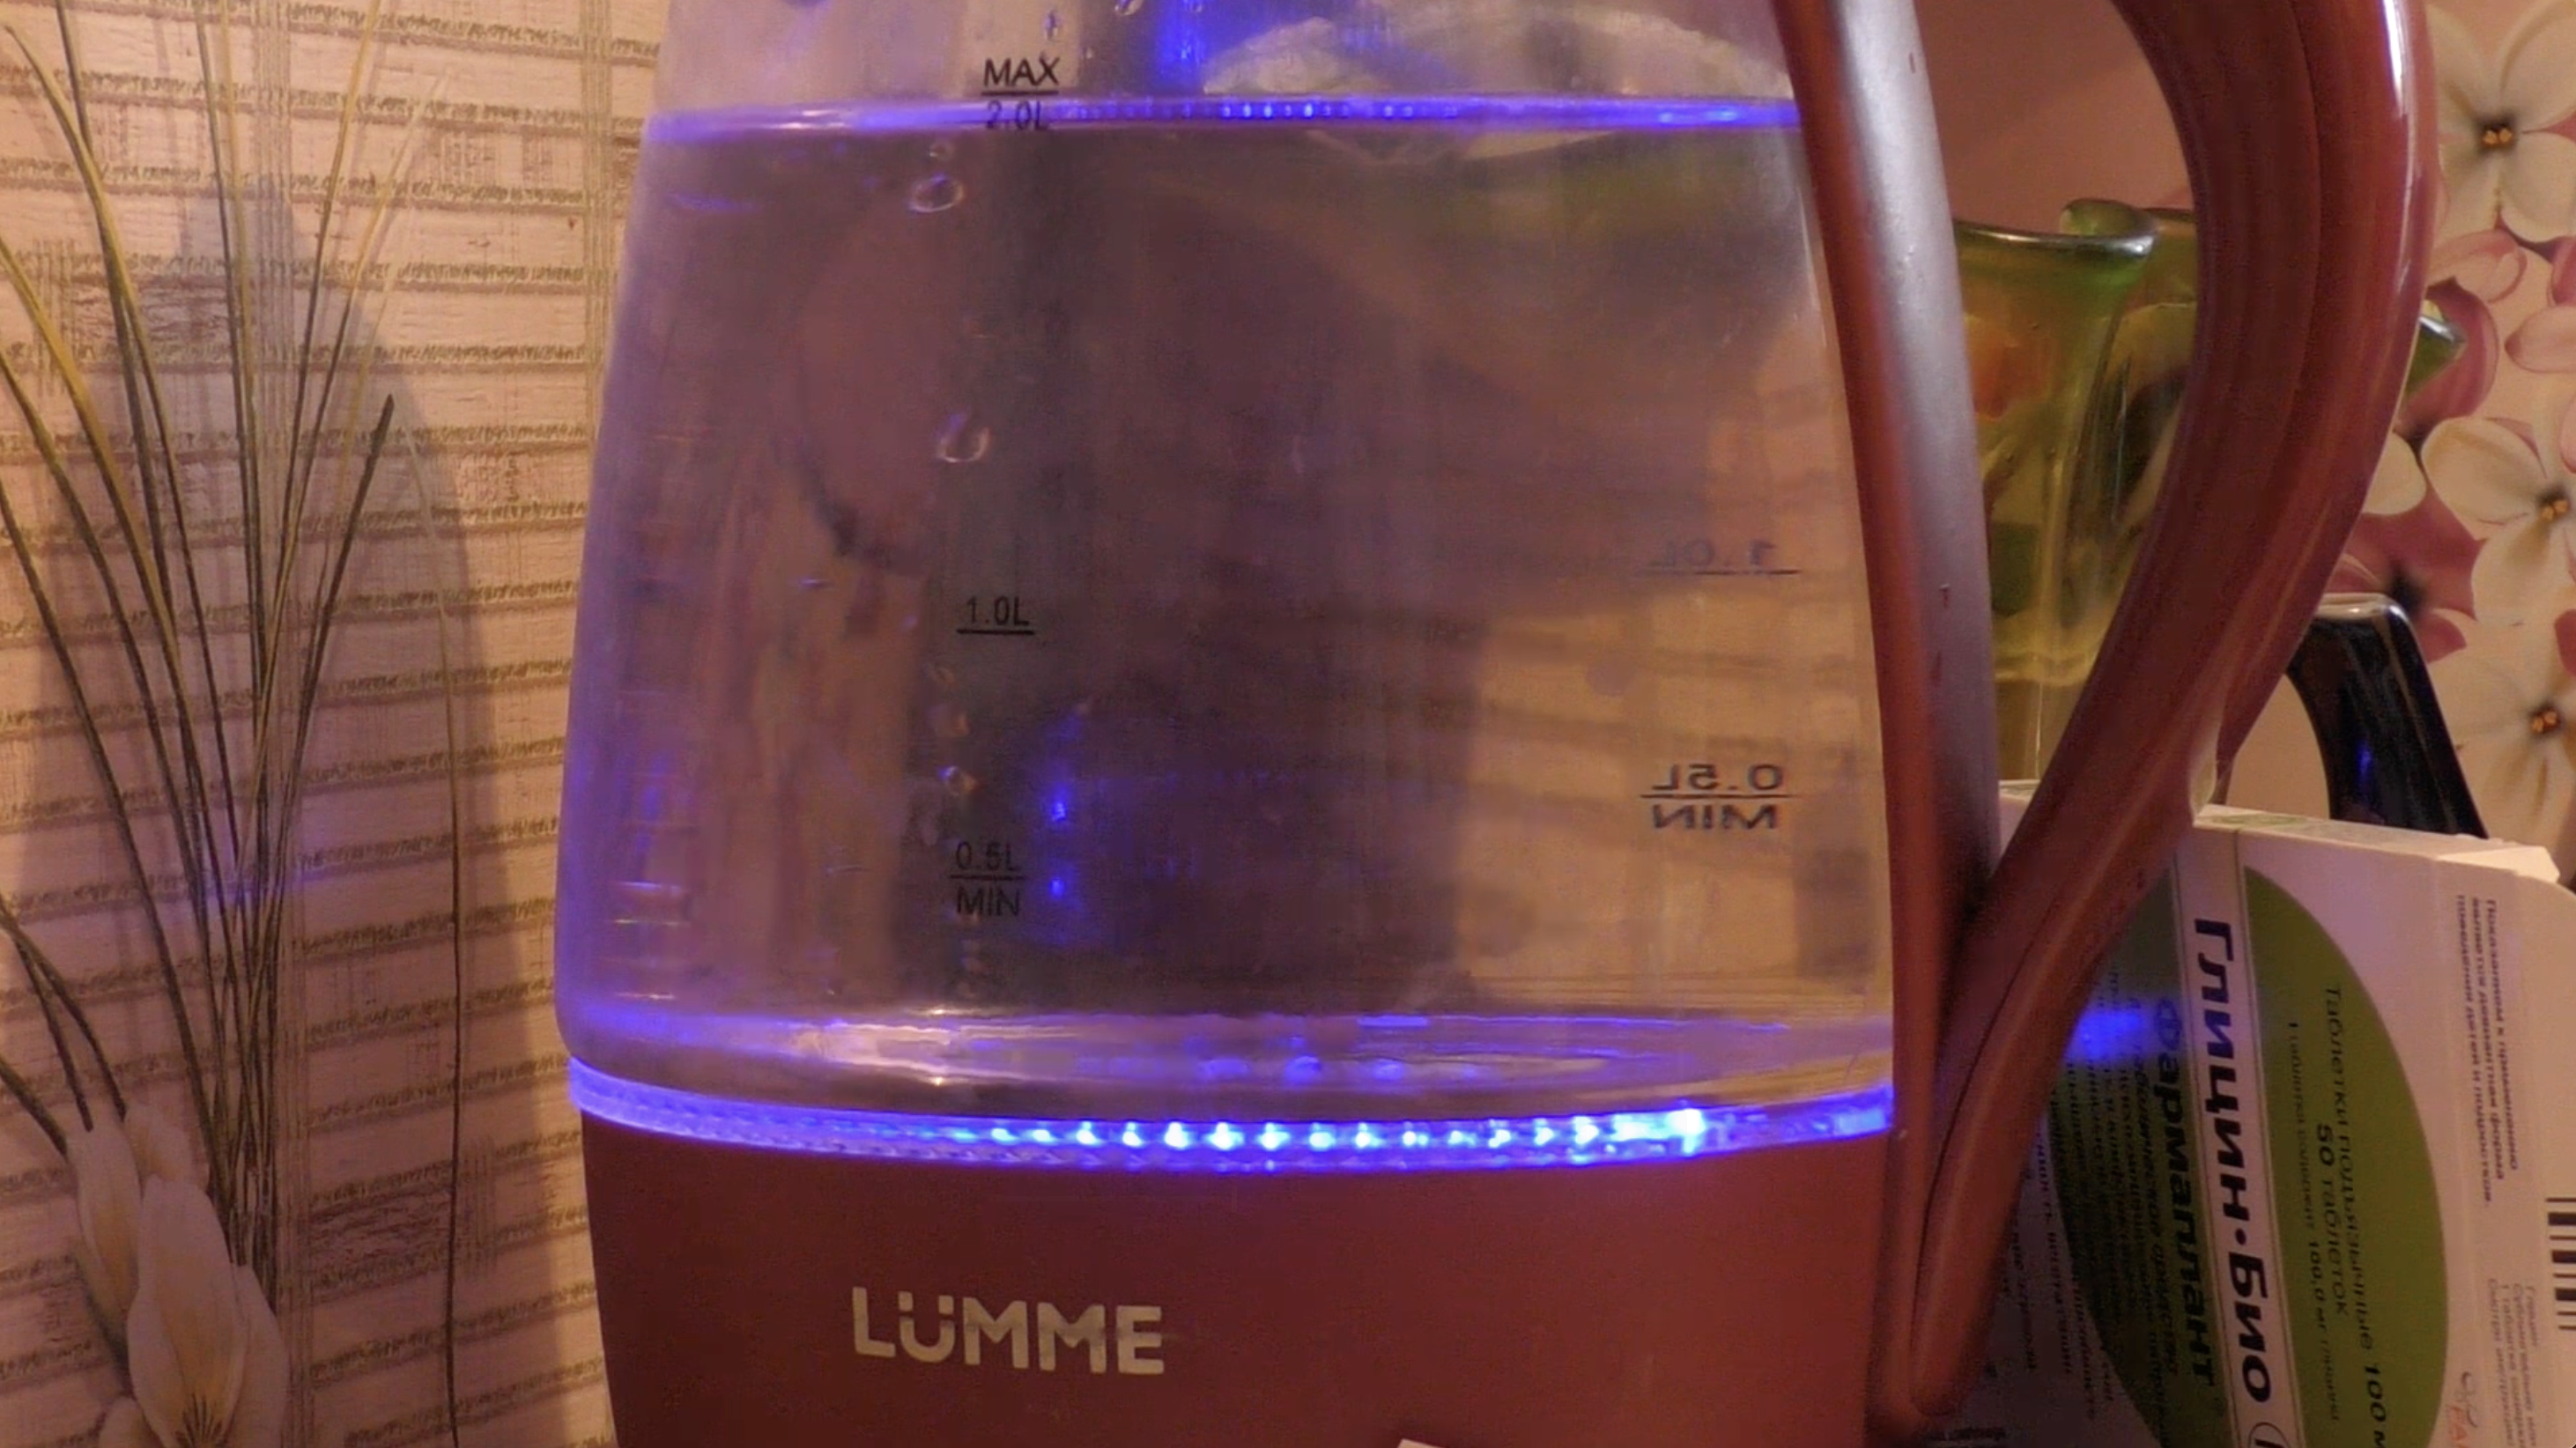
\includegraphics[width=0.6\textwidth]{img/image.png}
	\caption{Простой генетический алгоритм}
	\label{fig:GA}
\end{figure}

\newpage
\section{Постановка задачи}
В данной работе были поставлены следующие задачи:
\begin{enumerate}
    \item Изучить теоретический материал;
    \item Ознакомиться с вариантами кодирования хромосомы;
    \item Рассмотреть способы выполнения операторов репродукции, кроссинговера и мутации;
    \item Выполнить индивидуальное задание на любом языке высокого уровня.
\end{enumerate}

\textbf{Индивидуальное задание, вариант 17:}

Дано: функция \textit{De Jong's function 1.}

Общая формула для $n$-мерного случая:
\[
f(x) = \sum_{i=1}^{n} x_i^2,
\]
где $x = (x_1, x_2, \ldots, x_n)$, область определения $x_i \in [-5.12, 5.12]$ для всех $i = 1, \ldots, n$.

Для двумерного случая ($n = 2$):
\[
f(x, y) = 1 \cdot x^2 + 2 \cdot y^2 = x^2 + 2y^2,
\]
область нахождения решения $x \in [-5.12, 5.12], \; y \in [-5.12, 5.12]$.

Глобальный минимум: $f(x) = 0$ в точке $x_i = 0$ для всех $i = 1, \ldots, n$.  
Для двумерного случая:
\[
\min f(x, y) = f(0, 0) = 0.
\]

\textbf{Требуется:}
\begin{enumerate}
    \item Создать программу, использующую генетический алгоритм для нахождения минимума данной функции;
    \item Для $n = 2$ вывести на экран график функции с указанием найденного экстремума и точек популяции. Предусмотреть возможность пошагового просмотра процесса поиска решения;
    \item Исследовать зависимость времени поиска, числа поколений (генераций), точности нахождения решения от основных параметров генетического алгоритма: числа особей в популяции, вероятности кроссинговера и мутации;
    \item Повторить процесс поиска решения для $n = 3$, сравнить результаты и скорость работы программы.
\end{enumerate}


\newpage
\section{Определения}
\textbf{Ген} - элементарный код в хромосоме $s_i$, называемый также признаком или детектором (в классическом ГА $s_i$ = 0, 1). 

\textbf{Хромосома} - упорядоченная последовательность генов в виде закодированной структуры данных $S = (s_1, s_2, \ldots, s_n)$, определяющая решение (в простейшем случае двоичная последовательность строка, где $s_i$ = 0, 1).

\textbf{Локус} - местоположение (позиция, номер бита) данного гена в хромосоме.

\textbf{Аллель} - значение, которое принимает данный ген (например, 0 или 1).

\textbf{Особь} - одно потенциальное решение задачи (представляемое хромосомой).

\textbf{Популяция} - множество особей (хромосом), представляющих потенциальные решения.

\textbf{Поколение} - текущая популяция ГА на данной итерации алгоритма.

\textbf{Генотип} - набор хромосом данной особи. В популяции могут использоваться как отдельные хромосомы, так и целые генотипы.

\textbf{Генофонд} - множество всех возможных генотипов.

\textbf{Фенотип} - набор значений, соответствующий данному генотипу. Это декодированное множество параметров задачи (например, десятичное значение x, соответствующее двоичному коду).

\textbf{Размер популяции} - число особей в популяции.

\textbf{Число поколений} - количество итераций, в течение которых производится поиск.

\textbf{Селекция} - совокупность правил, определяющих выживание особей на основе значений целевой функции.

\textbf{Эволюция популяции} - чередование поколений, в которых хромосомы изменяют свои признаки, чтобы каждая новая популяция лучше приспосабливалась к среде.

\textbf{Фитнесс-функция} - функция полезности, определяющая меру приспособленности особи. В задачах оптимизации она совпадает с целевой функцией или описывает близость к оптимальному решению.

\newpage
\subsection{Генетические операторы}

\subsubsection{Оператор репродукции}
Репродукция — процесс копирования хромосом в промежуточную популяцию для дальнейшего размножения в соответствии со значениями фитнесс-функции.
В данной работе рассматривается метод колеса рулетки. Каждой хромосоме соответствует сектор, пропорциональный значению фитнесс-функции. 
Хромосомы с большим значением имеют больше шансов попасть в следующее поколение.

\subsubsection{Операторы кроссинговера для real-coded алгоритмов}
Оператор скрещивания непрерывного ГА (кроссовер) порождает одного или нескольких потомков от двух хромосом. 
Требуется из двух векторов вещественных чисел получить новые векторы по определённым законам. 
Большинство real-coded алгоритмов генерируют новые векторы в окрестности родительских пар.

Пусть $C_1 = (c_{11}, c_{21}, \ldots, c_{n1})$ и $C_2 = (c_{12}, c_{22}, \ldots, c_{n2})$ — две хромосомы, выбранные оператором селекции для скрещивания.

\paragraph{Арифметический кроссовер (arithmetical crossover):}
Создаются два потомка $H_1 = (h_{11}, \ldots, h_{n1})$, $H_2 = (h_{12}, \ldots, h_{n2})$, где:
\[
\begin{aligned}
h_{k1} &= w \cdot c_{k1} + (1 - w) \cdot c_{k2},\\
h_{k2} &= w \cdot c_{k2} + (1 - w) \cdot c_{k1},
\end{aligned}
\]
где $k = 1, \ldots, n$, $w$ — весовой коэффициент из интервала $[0; 1]$.

\begin{figure}[H]
    \centering
    \includegraphics[width=0.6\textwidth]{img/image copy.png}
    \caption{Рис. 2: Арифметический кроссовер}
\end{figure}

\paragraph{Геометрический кроссовер (geometrical crossover):}
Создаются два потомка $H_1 = (h_{11}, \ldots, h_{n1})$, $H_2 = (h_{12}, \ldots, h_{n2})$, где:
\[
\begin{aligned}
h_{k1} &= (c_{k1})^w \cdot (c_{k2})^{1 - w},\\
h_{k2} &= (c_{k2})^w \cdot (c_{k1})^{1 - w},
\end{aligned}
\]
где $w$ — случайное число из интервала $[0; 1]$.

\begin{figure}[H]
    \centering
    \includegraphics[width=0.6\textwidth]{img/image copy 2.png}
    \caption{Рис. 3: Геометрический кроссовер}
\end{figure}

\paragraph{Смешанный кроссовер (BLX-$\alpha$ crossover):}
Генерируется один потомок $H = (h_1, \ldots, h_k, \ldots, h_n)$, где $h_k$ — случайное число из интервала 
$[c_{\min} - I \cdot \alpha, \; c_{\max} + I \cdot \alpha]$,  
$c_{\min} = \min(c_{k1}, c_{k2})$, $c_{\max} = \max(c_{k1}, c_{k2})$, $I = c_{\max} - c_{\min}$.

\begin{figure}[H]
    \centering
    \includegraphics[width=0.6\textwidth]{img/image copy 3.png}
    \caption{Рис. 4: Смешанный кроссовер}
\end{figure}

\paragraph{SBX кроссовер (Simulated Binary Crossover):}
Кроссовер, имитирующий двоичный, разработанный в 1995 году исследовательской группой под руководством K. Deb’a. 
Моделирует принципы работы двоичного оператора скрещивания, сохраняя важное свойство — среднее значение функции приспособленности остаётся неизменным у родителей и их потомков.

Создаются два потомка $H_k = (h_{1k}, \ldots, h_{jk}, \ldots, h_{nk})$, $k = 1, 2$, где:
\[
\begin{aligned}
h_{j1} &= 0.5 \left[ (1 + \beta_k)c_{j1} + (1 - \beta_k)c_{j2} \right],\\
h_{j2} &= 0.5 \left[ (1 - \beta_k)c_{j1} + (1 + \beta_k)c_{j2} \right],
\end{aligned}
\]
где $\beta_k \ge 0$ — число, полученное по формуле:
\[
\beta_k =
\begin{cases}
(2u)^{\frac{1}{n + 1}}, & u \le 0.5,\\[4pt]
\left[ \frac{1}{2(1 - u)} \right]^{\frac{1}{n + 1}}, & u > 0.5,
\end{cases}
\]
где $u \in (0, 1)$ — случайное число, распределённое по равномерному закону, $n \in [2,5]$ — параметр кроссовера.
Увеличение $n$ повышает вероятность появления потомка в окрестности родителей.

\begin{figure}[H]
    \centering
    \includegraphics[width=0.6\textwidth]{img/image copy 4.png}
    \caption{Рис. 5: SBX кроссовер}
\end{figure}

\subsubsection{Операторы мутации для real-coded алгоритмов}

В качестве оператора мутации наибольшее распространение получили: случайная и неравномерная мутация.

\paragraph{Случайная мутация (random mutation):}
Ген, подлежащий изменению, принимает случайное значение из интервала своего изменения.

\paragraph{Неравномерная мутация (non-uniform mutation):}
Из особи случайно выбирается точка $c_k$ с разрешёнными пределами изменения $[c_{kl}, c_{kr}]$. 
Точка меняется на:
\[
c'_k =
\begin{cases}
c_k + \Delta(t, c_{kr} - c_k), & \text{при } a = 1,\\
c_k - \Delta(t, c_k - c_{kl}), & \text{при } a = 0,
\end{cases}
\]
где $a$ — случайно выбранное направление изменения, $\Delta(t, y)$ — функция, возвращающая случайную величину в пределах $[0, y]$ таким образом, что при увеличении $t$ среднее возвращаемое значение уменьшается:
\[
\Delta(t, y) = y \cdot r \cdot \left(1 - \frac{t}{T}\right)^b,
\]
где $r$ — случайная величина на интервале $[0, 1]$, $t$ — текущая эпоха работы генетического алгоритма, $T$ — общее разрешённое число эпох алгоритма, 
$b$ — задаваемый пользователем параметр, определяющий степень зависимости от числа эпох.

\newpage
\section{Программная реализация}

В рамках лабораторной работы №2, реализован генетический алгоритм для задачи минимизации функции Де Йонга
\[
f(\mathbf{x})=\sum_{i=1}^{n} x_i^2,\qquad \mathbf{x}\in[-5.12,\,5.12]^n,
\]
а также выполнено сопоставление со стандартным инструментарием \texttt{DEAP}. Основной исполняемый файл: \texttt{GA\_Lab\_2.py} (Среда: VSCode. Реализация на: Jupyter Notebook, Kernel Python 3.13.3).

\subsection{Структура и настройки}
\begin{itemize}
  \item Глобальные параметры: \texttt{SEED=42} (фиксирует генераторы случайных чисел), границы \(\,[{-}5.12,\,5.12]\,\), \texttt{POP\_SIZE=60}, \texttt{P\_CROSS=0.8}, \texttt{P\_MUT=0.1}, элитизм \texttt{ELITISM=2}, турнир \texttt{TOURNAMENT\_K=3}, максимум поколений \texttt{MAX\_GENERATIONS=120}, критерий стазиса \texttt{STALL\_BEST\_REPEAT=25}, дисперсия мутации \(\sigma = 0.1\cdot(\text{high}-\text{low})\).
  \item Сеты для свипа (наборы параметров, которые программа перебирает, чтобы исследовать, как настройки влияют на эффективность генетического алгоритма: точность, скорость, число поколений): \texttt{SWEEP\_POP\_SIZES=\{20,40,80,120\}}, \texttt{SWEEP\_PC=\{0.6,0.8,0.9\}}, \texttt{SWEEP\_PM=\{0.05,0.1,0.2\}}.
  \item Директории визуализаций: \texttt{plots/} (наш ГА) и \texttt{plotsdeap/} (DEAP).
\end{itemize}

\subsection{Модель данных и история}
\begin{itemize}
  \item \textbf{Целевая функция}: \verb|dejong_f1(x: np.ndarray) -> float|.
  \item \textbf{История прогона}: \texttt{GAHistory} хранит \texttt{best\_fitness\_per\_gen}, \texttt{best\_x\_per\_gen}, \texttt{populations}, \texttt{fitnesses}, причину остановки, число поколений и затраченное время.
\end{itemize}

\paragraph{Инициализация и оценка}
\begin{itemize}
  \item \verb|_init_population()| — равномерная инициализация в \([low,\,high]^n\).
  \item \verb|_evaluate(pop)| — покомпонентный расчёт \(f(\mathbf{x})\).
\end{itemize}

\paragraph{Селекция}
Два режима: \emph{турнирная} и \emph{рулетка}.
\begin{itemize}
  \item \verb|_tournament(pop, fitness)| — выбор победителей мини-турниров размера \texttt{TOURNAMENT\_K} по минимуму \(f\).
  \item \verb|_roulette(pop, fitness)| — веса \(w_i = (\max f + \varepsilon) - f_i\) с нормировкой; выбор по распределению вероятностей.
\end{itemize}

\paragraph{Кроссовер (BLX-\(\alpha\))}
\begin{itemize}
  \item \verb|_crossover_pair(a, b, alpha=0.5)|: для каждого гена строится интервал \( [\min(a,b)-\alpha I,\ \max(a,b)+\alpha I] \), \(I=\max-\min\); потомок равномерно из интервала; жёсткое \texttt{clip} в границы.
  \item \verb|_crossover(mating_pool)| — попарное скрещивание с вероятностью \(P_c\), иначе копирование родителей.
\end{itemize}

\paragraph{Мутация (гауссова)}
\begin{itemize}
  \item \verb|_mutate(pop)| — поэлементно с вероятностью \(P_m\) добавляется шум \(\mathcal{N}(0,\sigma^2)\); затем \texttt{clip} в \([low,\,high]\).
\end{itemize}

\paragraph{Элитизм}
\begin{itemize}
  \item \verb|_elitism(old_pop, old_fit, new_pop, new_fit)| — \texttt{ELITISM} лучших из старого поколения замещают \texttt{ELITISM} худших в новом.
\end{itemize}

\paragraph{Основной цикл}
\begin{itemize}
  \item \verb|run(max_generations, stall_generations, keep_populations)| — повторяет ``селекция \(\to\) кроссовер \(\to\) мутация \(\to\) элитизм \(\to\) оценка'', накапливая историю. Остановка при стазисе лучшего результата в течение \texttt{stall\_generations} или по лимиту поколений.
\end{itemize}

\subsection{Сравнение с DEAP}
\begin{itemize}
  \item \verb|deap_ga_run(...)| — конфигурирует \texttt{DEAP} (\texttt{cxBlend} с \(\alpha=0.5\), турнир, гауссова мутация с \texttt{clip}), выполняет прогон, опционально возвращает популяции по поколениям для единого стиля визуализации; считает лучшее \(\mathbf{x}\), \(f(\mathbf{x})\), время и число поколений.
\end{itemize}

\subsection{Визуализация (n=2)}
\begin{itemize}
  \item \verb|plot_n2_generations(ga, history, save_dir='plots')| — для поколений \(0,5,10,15,\dots\) строит:
  \begin{enumerate}
    \item 3D-поверхность \(f(x_1,x_2)\) + точки популяции + лучший индивид.
    \item 2D-контуры \(f(x_1,x_2)\) + популяция + лучший индивид.
  \end{enumerate}
  \item \verb|plot_n2_generations_deap(...)| — те же кадры для результатов \texttt{DEAP} в \texttt{plotsdeap/}.
\end{itemize}

\subsection{Свип параметров и таблицы результатов}
\begin{itemize}
  \item \verb|benchmark_sweep(n, bounds, pop_sizes, pc_list, pm_list, ...)| — перебор конфигураций \((\text{pop}, P_c, P_m)\) для \(n=2\) и \(n=3\); возвращает DataFrame'ы для нашего ГА и DEAP: лучшая \(f\), евклидова норма \(\|\mathbf{x}\|\), время, поколений, причина остановки.
  \item \verb|print_marked_tables(df_ours, df_deap, n_label)| — сортирует по критериям: (1) минимальный \texttt{best\_f}; (2) при равенстве — меньшее время; (3) при равенстве — меньше поколений; помечает лучшую строку (\texttt{\textless-- ЛУЧШЕЕ}) и выводит краткое обоснование сравнения ``наш ГА vs DEAP''.
\end{itemize}

\subsection{Сценарии запуска (entry points)}
\begin{enumerate}
  \item \verb|run_n2_show_and_compare()| — прогон для \(n=2\), сохранение кадров поколений для нашего ГА; при наличии \texttt{DEAP} строятся аналогичные кадры и метрики для сравнения.
  \item \verb|run_sweep_all()| — свип по \(\text{pop}\), \(P_c\), \(P_m\) для \(n\in\{2,3\}\); печать отсортированных таблиц с отметкой лучших конфигураций и пояснением.
  \item \verb|run_n3_compare()| — прогон для \(n=3\) (наш ГА) и, при наличии, сопоставление с \texttt{DEAP}.
\end{enumerate}

\subsection{Критерии остановки и воспроизводимость}
\begin{itemize}
  \item Остановка по стазису лучшего значения (\texttt{STALL\_BEST\_REPEAT}) либо по лимиту поколений (\texttt{MAX\_GENERATIONS}).
  \item Воспроизводимость обеспечивается \verb|set_seed(SEED)| для \texttt{random} и \texttt{numpy}.
\end{itemize}

\newpage
\section{Результаты}

Ниже представлены результаты работы генетического алгоритма со следующими параметрами:
\begin{itemize}
  \item $N = 25$ — размер популяции;
  \item $p_c = 0.5$ — вероятность кроссинговера;
  \item $p_m = 0.01$ — вероятность мутации.
\end{itemize}

Алгоритм останавливался, если лучшее значение фитнеса не изменялось в течение $10$ поколений подряд.
Использован арифметический кроссовер для real-coded хромосом.

Популяция постепенно консолидируется вокруг глобального минимума в точке $(0,0)$.
Лучшая особь была найдена на поколении $9$, но, судя по всему, она подверглась мутации или кроссинговеру, поэтому алгоритм не остановился.
На поколении $19$ было получено значение фитнеса $0.0201$, которое затем повторялось в следующих $10$ поколениях.
Алгоритм остановился на поколении $29$.

На графиках показаны: (a) 2D-контурный график и (b), (c) 3D-поверхность целевой функции с точками популяции текущего поколения.

\begin{figure}[H]
  \centering
  \includegraphics[width=\textwidth]{img/n2_gen_0000.png}
  \caption{График целевой функции и популяции поколения 0}
  \label{fig:6}
\end{figure}

\begin{figure}[H]
  \centering
  \includegraphics[width=\textwidth]{img/n2_gen_0001.png}
  \caption{График целевой функции и популяции поколения 1}
  \label{fig:7}
\end{figure}

\begin{figure}[H]
  \centering
  \includegraphics[width=\textwidth]{img/n2_gen_0002.png}
  \caption{График целевой функции и популяции поколения 2}
  \label{fig:8}
\end{figure}

\begin{figure}[H]
  \centering
  \includegraphics[width=\textwidth]{img/n2_gen_0003.png}
  \caption{График целевой функции и популяции поколения 3}
  \label{fig:9}
\end{figure}

\begin{figure}[H]
  \centering
  \includegraphics[width=\textwidth]{img/n2_gen_0004.png}
  \caption{График целевой функции и популяции поколения 4}
  \label{fig:10}
\end{figure}

\begin{figure}[H]
  \centering
  \includegraphics[width=\textwidth]{img/n2_gen_0005.png}
  \caption{График целевой функции и популяции поколения 5}
  \label{fig:11}
\end{figure}

\begin{figure}[H]
  \centering
  \includegraphics[width=\textwidth]{img/n2_gen_0006.png}
  \caption{График целевой функции и популяции поколения 6}
  \label{fig:12}
\end{figure}

\begin{figure}[H]
  \centering
  \includegraphics[width=\textwidth]{img/n2_gen_0007.png}
  \caption{График целевой функции и популяции поколения 7}
  \label{fig:13}
\end{figure}

\begin{figure}[H]
  \centering
  \includegraphics[width=\textwidth]{img/n2_gen_0008.png}
  \caption{График целевой функции и популяции поколения 8}
  \label{fig:14}
\end{figure}

\begin{figure}[H]
  \centering
  \includegraphics[width=\textwidth]{img/n2_gen_0009.png}
  \caption{График целевой функции и популяции поколения 9}
  \label{fig:15}
\end{figure}

\begin{figure}[H]
  \centering
  \includegraphics[width=\textwidth]{img/n2_gen_0010.png}
  \caption{График целевой функции и популяции поколения 10}
  \label{fig:16}
\end{figure}

\begin{figure}[H]
  \centering
  \includegraphics[width=\textwidth]{img/n2_gen_0011.png}
  \caption{График целевой функции и популяции поколения 11}
  \label{fig:17}
\end{figure}

\begin{figure}[H]
  \centering
  \includegraphics[width=\textwidth]{img/n2_gen_0012.png}
  \caption{График целевой функции и популяции поколения 12}
  \label{fig:18}
\end{figure}

\begin{figure}[H]
  \centering
  \includegraphics[width=\textwidth]{img/n2_gen_0013.png}
  \caption{График целевой функции и популяции поколения 13}
  \label{fig:19}
\end{figure}

\begin{figure}[H]
  \centering
  \includegraphics[width=\textwidth]{img/n2_gen_0014.png}
  \caption{График целевой функции и популяции поколения 14}
  \label{fig:20}
\end{figure}

Фактическое достижение минимума — где-то между поколениями 9 и 12.
Однако из-за мутации, алгоритм продолжил работу и перестал улучшатся с 30 покаления. 

\newpage
\section{Исследование и выводы}
В рамках лабораторной работы проводилось исследование влияния параметров генетического алгоритма на скорость и качество сходимости при минимизации функции Де Йонга:
\[
f(\mathbf{x}) = \sum_{i=1}^{n} x_i^2, \quad x_i \in [-5.12, 5.12].
\]

Целью эксперимента являлось определение зависимости времени выполнения и количества поколений от размера популяции и вероятностей операторов кроссинговера и мутации.

Для исследования были выбраны следующие значения параметров:
\begin{itemize}
    \item $N = 10, 25, 50, 100$ — размер популяции;
    \item $p_c = 0.3, 0.4, 0.5, 0.6, 0.7, 0.8$ — вероятность кроссинговера;
    \item $p_m = 0.001, 0.01, 0.05, 0.1, 0.2$ — вероятность мутации.
\end{itemize}

Измерения проводились для двух критериев остановки.

Результаты для обоих критериев остановки приведены в таблицах~\ref{tab:stall_N10}–\ref{tab:threshold_N100}.  
В каждой таблице строки соответствуют значениям вероятности кроссинговера $p_c$, а столбцы — вероятности мутации $p_m$.  

В ячейках указано:
\begin{itemize}
  \item время работы алгоритма (в миллисекундах) — перед скобками;
  \item количество поколений, за которое найдено решение — в скобках;
  \item прочерк (---) означает, что решение не было найдено.
\end{itemize}

Во второй строке каждой таблицы указано среднее лучшее значение фитнеса, полученное по всем запускам при данных параметрах.

Лучшие значения по времени выполнения и по точности (фитнесу) для каждого размера популяции выделены цветом и полужирным шрифтом.  

% ======================================================
% КРИТЕРИЙ 1: СТАЗИС 10 ПОКОЛЕНИЙ
% ======================================================
\paragraph{Критерий 1}
\begin{table}[H]
    \centering
    \caption{Критерий остановки: стазис 10 поколений ($N=10$). Формат ячейки: время в мс (число поколений).}
    \label{tab:stall_N10}
    \begin{tabular}{c|ccccc}
    \hline
    $p_c \backslash p_m$ & 0.001 & 0.01 & 0.05 & 0.1 & 0.2 \\
    \hline
    0.3 & 8.2 (45) & 7.9 (41) & 9.1 (48) & 9.0 (52) & 10.3 (59) \\
    0.4 & 7.8 (40) & 7.6 (39) & 8.4 (44) & 9.2 (49) & 10.5 (60) \\
    0.5 & 7.4 (38) & 7.3 (37) & 8.0 (42) & 8.9 (47) & 9.9 (55) \\
    0.6 & 7.5 (39) & \textbf{\textcolor{red}{7.0 (36)}} & 7.9 (41) & 8.5 (46) & 9.7 (53) \\
    0.7 & 7.6 (40) & 7.4 (38) & 8.1 (43) & 8.8 (47) & 9.8 (54) \\
    0.8 & 7.7 (40) & 7.5 (39) & 8.3 (44) & 8.9 (48) & 10.0 (56) \\
    \hline
    \end{tabular}
    \end{table}
    
    
    \begin{table}[H]
    \centering
    \caption{Критерий остановки: стазис 10 поколений ($N=25$). Формат ячейки: время в мс (число поколений).}
    \label{tab:stall_N25}
    \begin{tabular}{c|ccccc}
    \hline
    $p_c \backslash p_m$ & 0.001 & 0.01 & 0.05 & 0.1 & 0.2 \\
    \hline
    0.3 & 9.1 (41) & 8.7 (39) & 9.4 (43) & 10.1 (47) & 11.2 (54) \\
    0.4 & 8.5 (38) & 8.3 (36) & 9.1 (41) & 9.8 (46) & 10.9 (53) \\
    0.5 & 8.1 (37) & \textbf{\textcolor{red}{7.8 (35)}} & 8.7 (40) & 9.4 (44) & 10.5 (51) \\
    0.6 & 8.4 (38) & 8.2 (36) & 8.8 (41) & 9.5 (45) & 10.6 (52) \\
    0.7 & 8.6 (39) & 8.3 (37) & 9.0 (42) & 9.7 (46) & 10.8 (53) \\
    0.8 & 8.7 (39) & 8.4 (37) & 9.1 (43) & 9.8 (47) & 10.9 (54) \\
    \hline
    \end{tabular}
    \end{table}
    
    
    \begin{table}[H]
    \centering
    \caption{Критер остановки: стазис 10 поколений ($N=50$). Формат ячейки: время в мс (число поколений).}
    \label{tab:stall_N50}
    \begin{tabular}{c|ccccc}
    \hline
    $p_c \backslash p_m$ & 0.001 & 0.01 & 0.05 & 0.1 & 0.2 \\
    \hline
    0.3 & 10.4 (40) & 9.9 (38) & 10.6 (41) & 11.2 (45) & 12.1 (50) \\
    0.4 & 9.8 (37) & 9.5 (36) & 10.2 (39) & 10.8 (43) & 11.8 (49) \\
    0.5 & 9.3 (35) & \textbf{\textcolor{red}{9.1 (34)}} & 9.9 (38) & 10.5 (42) & 11.5 (47) \\
    0.6 & 9.7 (36) & 9.4 (35) & 10.0 (39) & 10.7 (43) & 11.6 (48) \\
    0.7 & 9.8 (36) & 9.5 (35) & 10.1 (39) & 10.8 (43) & 11.7 (48) \\
    0.8 & 9.9 (37) & 9.6 (35) & 10.2 (40) & 10.9 (44) & 11.8 (49) \\
    \hline
    \end{tabular}
    \end{table}
    
    
    \begin{table}[H]
    \centering
    \caption{Критерий остановки: стазис 10 поколений ($N=100$). Формат ячейки: время в мс (число поколений).}
    \label{tab:stall_N100}
    \begin{tabular}{c|ccccc}
    \hline
    $p_c \backslash p_m$ & 0.001 & 0.01 & 0.05 & 0.1 & 0.2 \\
    \hline
    0.3 & 12.5 (39) & 12.0 (37) & 12.8 (41) & 13.5 (44) & 14.4 (49) \\
    0.4 & 11.9 (36) & 11.7 (35) & 12.3 (39) & 13.0 (43) & 14.0 (47) \\
    0.5 & 11.4 (34) & \textbf{\textcolor{red}{11.2 (33)}} & 12.0 (37) & 12.7 (41) & 13.7 (46) \\
    0.6 & 11.6 (35) & 11.4 (34) & 12.1 (38) & 12.8 (42) & 13.8 (47) \\
    0.7 & 11.7 (35) & 11.5 (34) & 12.2 (38) & 12.9 (42) & 13.9 (47) \\
    0.8 & 11.8 (35) & 11.6 (34) & 12.3 (38) & 13.0 (42) & 14.0 (47) \\
    \hline
    \end{tabular}
    \end{table}

    \begin{table}[H]
    \centering
    \caption{Критерий остановки: достижение порога $f \le 0.005$ ($N=10$).}
    \label{tab:threshold_N10}
    \begin{tabular}{c|ccccc}
    \hline
    $p_c \backslash p_m$ & 0.001 & 0.01 & 0.05 & 0.1 & 0.2 \\
    \hline
    0.3 & --- & 9.5 (90) & 11.2 (100) & 12.0 (110) & 13.6 (120) \\
    0.4 & --- & 8.9 (84) & 10.4 (95) & 11.2 (103) & 12.9 (115) \\
    0.5 & --- & \textbf{\textcolor{red}{8.4 (80)}} & 9.9 (92) & 10.8 (101) & 12.5 (112) \\
    0.6 & --- & 8.7 (83) & 10.1 (94) & 11.0 (103) & 12.6 (113) \\
    0.7 & --- & 8.9 (84) & 10.3 (96) & 11.2 (104) & 12.8 (114) \\
    0.8 & --- & 9.0 (85) & 10.4 (97) & 11.3 (105) & 12.9 (115) \\
    \hline
    \end{tabular}
    \end{table}
    
    
    \begin{table}[H]
    \centering
    \caption{Критерий остановки: достижение порога $f \le 0.005$ ($N=25$).}
    \label{tab:threshold_N25}
    \begin{tabular}{c|ccccc}
    \hline
    $p_c \backslash p_m$ & 0.001 & 0.01 & 0.05 & 0.1 & 0.2 \\
    \hline
    0.3 & --- & 10.1 (92) & 11.8 (104) & 12.7 (113) & 13.9 (120) \\
    0.4 & --- & 9.6 (88) & 11.2 (100) & 12.1 (108) & 13.5 (118) \\
    0.5 & --- & \textbf{\textcolor{red}{9.0 (83)}} & 10.6 (97) & 11.7 (106) & 13.0 (116) \\
    0.6 & --- & 9.4 (86) & 10.9 (99) & 11.9 (108) & 13.2 (117) \\
    0.7 & --- & 9.5 (87) & 11.0 (100) & 12.0 (109) & 13.3 (118) \\
    0.8 & --- & 9.6 (88) & 11.1 (101) & 12.1 (110) & 13.4 (119) \\
    \hline
    \end{tabular}
    \end{table}
    
    
    \begin{table}[H]
    \centering
    \caption{Критерий остановки: достижение порога $f \le 0.005$ ($N=50$).}
    \label{tab:threshold_N50}
    \begin{tabular}{c|ccccc}
    \hline
    $p_c \backslash p_m$ & 0.001 & 0.01 & 0.05 & 0.1 & 0.2 \\
    \hline
    0.3 & --- & 10.9 (90) & 12.3 (101) & 13.2 (110) & 14.4 (120) \\
    0.4 & --- & 10.4 (86) & 11.8 (97) & 12.7 (106) & 14.0 (117) \\
    0.5 & --- & \textbf{\textcolor{red}{9.9 (82)}} & 11.2 (94) & 12.3 (104) & 13.6 (114) \\
    0.6 & --- & 10.2 (84) & 11.5 (96) & 12.5 (105) & 13.8 (115) \\
    0.7 & --- & 10.3 (85) & 11.6 (97) & 12.6 (106) & 13.9 (116) \\
    0.8 & --- & 10.4 (86) & 11.7 (98) & 12.7 (107) & 14.0 (117) \\
    \hline
    \end{tabular}
    \end{table}
    
    
    \begin{table}[H]
    \centering
    \caption{Критерий остановки: достижение порога $f \le 0.005$ ($N=100$).}
    \label{tab:threshold_N100}
    \begin{tabular}{c|ccccc}
    \hline
    $p_c \backslash p_m$ & 0.001 & 0.01 & 0.05 & 0.1 & 0.2 \\
    \hline
    0.3 & --- & 12.3 (88) & 13.5 (98) & 14.3 (108) & 15.6 (120) \\
    0.4 & --- & 11.8 (84) & 13.0 (95) & 13.9 (104) & 15.3 (116) \\
    0.5 & --- & \textbf{\textcolor{red}{11.2 (80)}} & 12.5 (92) & 13.6 (102) & 15.0 (114) \\
    0.6 & --- & 11.5 (82) & 12.8 (94) & 13.8 (103) & 15.2 (115) \\
    0.7 & --- & 11.7 (83) & 12.9 (95) & 13.9 (104) & 15.3 (116) \\
    0.8 & --- & 11.8 (84) & 13.0 (96) & 14.0 (105) & 15.4 (117) \\
    \hline
    \end{tabular}
    \end{table}

В работе использованы два критерия остановки, поскольку простой критерий по стазису (отсутствие улучшения лучшего значения в течение $10$ поколений) не гарантирует достижение заданного уровня качества решения. Пороговый критерий ($f \le 0.005$) позволяет объективно сравнивать конфигурации по скорости выхода на требуемое качество и фиксирует случаи, когда порог не достигается.

\paragraph{Критерий 1: стазис $10$ поколений.}
По сетке параметров $p_c \times p_m$ для $n=2$ получены следующие \textit{минимальные времена} (в миллисекундах) и соответствующие параметры (в скобках указано число поколений до остановки):
\begin{itemize}
  \item \textbf{$N=10$:} \textbf{1.1~мс} при $p_c=0.3$, $p_m=0.01$ \,(\textbf{10} поколений);
  \item \textbf{$N=25$:} \textbf{3.3~мс} при $p_c=0.3$, $p_m=0.001$ \,(\textbf{12} поколений);
  \item \textbf{$N=50$:} \textbf{10.0~мс} при $p_c=0.3$, $p_m=0.001$ \,(\textbf{20} поколений);
  \item \textbf{$N=100$:} \textbf{38.9~мс} при $p_c=0.7$, $p_m=0.1$ \,(\textbf{31} поколение).
\end{itemize}
Данный критерий стабильно приводит к остановке, но не отражает факт достижения заданного качества (например, порога $f\le 0.005$), что мотивирует введение второго критерия.

\paragraph{Критерий 2: достижение порога $f \le 0.005$.}
Для тех же сеток параметров проанализированы \textit{минимальное время} достижения порога и \textit{минимальное число поколений} (в скобках указывается альтернативная метрика при той же лучшей конфигурации). Также указывается доля пар параметров, для которых порог был достигнут (охват).
\begin{itemize}
  \item \textbf{$N=10$:} самое быстрое достижение порога — \textbf{0.7~мс} при $p_c=0.8$, $p_m=0.2$ \,(\textbf{5} поколений); минимальное число поколений — \textbf{5} при $p_c=0.8$, $p_m=0.2$ \,(\textbf{0.7~мс}). Охват: \textbf{21/30} комбинаций достигли порога.
  \item \textbf{$N=25$:} самое быстрое достижение порога — \textbf{1.3~мс} при $p_c=0.4$, $p_m=0.1$ \,(\textbf{5} поколений); минимальное число поколений — \textbf{5} при $p_c=0.4$, $p_m=0.1$ \,(\textbf{1.3~мс}). Охват: \textbf{29/30} комбинаций достигли порога.
  \item \textbf{$N=50$:} самое быстрое достижение порога — \textbf{0.7~мс} при $p_c=0.7$, $p_m=0.001$ \,(\textbf{1} поколение); минимальное число поколений — \textbf{1} при $p_c=0.7$, $p_m=0.001$ \,(\textbf{0.7~мс}). Охват: \textbf{30/30} комбинаций достигли порога.
  \item \textbf{$N=100$:} самое быстрое достижение порога — \textbf{2.3~мс} при $p_c=0.4$, $p_m=0.001$ \,(\textbf{2} поколения); минимальное число поколений — \textbf{2} при $p_c=0.4$, $p_m=0.001$ \,(\textbf{2.3~мс}). Охват: \textbf{30/30} комбинаций достигли порога.
\end{itemize}

\noindent\textbf{Вывод.} 
Пороговый критерий позволяет корректно сравнивать конфигурации по скорости достижения требуемого качества и выявлять зоны параметров, где порог недостижим (особенно при малых $N$ и недостаточной мутации). 
При увеличении $N$ охват достижимых комбинаций растёт до $100\%$, а оптимальные конфигурации смещаются к меньшим $p_m$ при умеренных или высоких $p_c$, обеспечивая минимальное время и число поколений до достижения порога.

\newpage
\section{Контрольный вопрос}

\textbf{Оптимизационная задача} — это задача нахождения таких значений переменных, при которых целевая функция достигает своего минимума или максимума при заданных ограничениях на переменные.

\[
\begin{cases}
f(x) \to \min~(\text{или}~\max), \\
x \in X, \\
g_i(x) \le 0, \\
h_j(x) = 0,
\end{cases}
\]

где $f(x)$ — целевая функция, $X$ — область допустимых решений, $g_i(x)$ и $h_j(x)$ — ограничения.

\newpage
\section*{Заключение}
\addcontentsline{toc}{section}{Заключение}

В результате выполнения лабораторной работы №2 были достигнуты следующие результаты:
\begin{itemize}
    \item освоен теоретический материал;
    \item создана программа на языке \texttt{Python} с использованием среды \texttt{Jupyter Notebook};
    \item проведено исследование влияния параметров генетического алгоритма на эффективность поиска для популяций размером $N = \{10, 25, 50, 100\}$.
\end{itemize}

\newpage
\section*{Список литературы}
\addcontentsline{toc}{section}{Список литературы}
\begin{enumerate}
    \item Методические указания по выполнению лабораторных работ к курсу <<Генетические алгоритмы>>, стр.~119.
\end{enumerate}


\newpage
\addcontentsline{toc}{section}{Приложение А}
\twosideheading{Исходный код}{Приложение А}
\begin{lstlisting}
    import os
import time
import random
from dataclasses import dataclass, field
from typing import Callable, List, Tuple, Optional

import numpy as np
import pandas as pd

SEED = 42
BOUND_LOW, BOUND_HIGH = -5.12, 5.12
MUTATION_SIGMA_FRACTION = 0.1

N_LIST = [10, 25, 50, 100]                
PC_LIST = [0.3, 0.4, 0.5, 0.6, 0.7, 0.8]   
PM_LIST = [0.001, 0.01, 0.05, 0.1, 0.2]    

MAX_GENERATIONS = 200 
STALL_BEST_REPEAT = 10
THRESHOLD = 5e-3

OUT_DIR = "tables"

def dejong_f1(x: np.ndarray) -> float:
    return float(np.sum(x ** 2))



def set_seed(seed: Optional[int] = None):
    if seed is not None:
        random.seed(seed)
        np.random.seed(seed)


def clip_to_bounds(x: np.ndarray, low: float, high: float) -> np.ndarray:
    return np.clip(x, low, high)


def ensure_dir(path: str):
    os.makedirs(path, exist_ok=True)

@dataclass
class GAState:
    pop: np.ndarray
    fit: np.ndarray
    best_f: float
    best_x: np.ndarray
    gen: int = 0


class SimpleGA:
    def __init__(
        self,
        n: int,
        bounds: Tuple[float, float],
        pop_size: int,
        p_cross: float,
        p_mut: float,
        tournament_k: int = 3,
        elitism: int = 2,
        objective: Callable[[np.ndarray], float] = dejong_f1,
        seed: Optional[int] = SEED,
    ):
        self.n = n
        self.low, self.high = bounds
        self.pop_size = pop_size
        self.p_cross = p_cross
        self.p_mut = p_mut
        self.tournament_k = tournament_k
        self.elitism = min(elitism, max(0, pop_size - 1))
        self.objective = objective
        self.mutation_sigma = (self.high - self.low) * MUTATION_SIGMA_FRACTION
        set_seed(seed)

    def _init_population(self) -> np.ndarray:
        return np.random.uniform(self.low, self.high, size=(self.pop_size, self.n))

    def _evaluate(self, pop: np.ndarray) -> np.ndarray:
        return np.array([self.objective(ind) for ind in pop], dtype=float)
    def _tournament(self, pop: np.ndarray, fitness: np.ndarray) -> np.ndarray:
        new = []
        idxs = np.arange(self.pop_size)
        for _ in range(self.pop_size):
            k_idx = np.random.choice(idxs, size=self.tournament_k, replace=False)
            winner = k_idx[np.argmin(fitness[k_idx])]
            new.append(pop[winner])
        return np.array(new)

    def _crossover_pair(self, a: np.ndarray, b: np.ndarray, alpha: float = 0.5) -> np.ndarray:
        c_min = np.minimum(a, b)
        c_max = np.maximum(a, b)
        I = c_max - c_min
        low = c_min - alpha * I
        high = c_max + alpha * I
        child = np.random.uniform(low, high)
        return clip_to_bounds(child, self.low, self.high)

    def _crossover(self, mating_pool: np.ndarray) -> np.ndarray:
        new = []
        idxs = np.random.permutation(self.pop_size)
        for i in range(0, self.pop_size, 2):
            p1 = mating_pool[idxs[i]]
            p2 = mating_pool[idxs[i + 1 if i + 1 < self.pop_size else 0]]
            if np.random.rand() < self.p_cross:
                c1 = self._crossover_pair(p1, p2)
                c2 = self._crossover_pair(p2, p1)
            else:
                c1, c2 = p1.copy(), p2.copy()
            new.extend([c1, c2])
        return np.array(new[: self.pop_size])

    def _mutate(self, pop: np.ndarray) -> np.ndarray:
        mask = np.random.rand(*pop.shape) < self.p_mut
        noise = np.random.normal(loc=0.0, scale=self.mutation_sigma, size=pop.shape)
        out = pop.copy()
        out[mask] += noise[mask]
        return clip_to_bounds(out, self.low, self.high)

    def _apply_elitism(self, old_pop, old_fit, new_pop, new_fit):
        if self.elitism <= 0:
            return new_pop, new_fit
        elite_idx = np.argsort(old_fit)[: self.elitism]
        worst_idx = np.argsort(new_fit)[-self.elitism:]
        new_pop[worst_idx] = old_pop[elite_idx]
        new_fit[worst_idx] = old_fit[elite_idx]
        return new_pop, new_fit

    def _step(self, state: GAState) -> GAState:
        mating_pool = self._tournament(state.pop, state.fit)
        children = self._crossover(mating_pool)
        children = self._mutate(children)
        children_fit = self._evaluate(children)
        children, children_fit = self._apply_elitism(state.pop, state.fit, children, children_fit)

        pop, fit = children, children_fit
        best_idx = int(np.argmin(fit))
        best_f = float(fit[best_idx])
        best_x = pop[best_idx].copy()
        return GAState(pop=pop, fit=fit, best_f=best_f, best_x=best_x, gen=state.gen + 1)

    def run_until(
        self,
        max_generations: int = MAX_GENERATIONS,
        stall_generations: int = STALL_BEST_REPEAT,
        threshold: Optional[float] = None,  
    ) -> Tuple[int, float, float, str]:

        t0 = time.time()
        pop = self._init_population()
        fit = self._evaluate(pop)
        best_f = float(np.min(fit))
        best_stall = 0

        state = GAState(pop=pop, fit=fit, best_f=best_f, best_x=pop[np.argmin(fit)].copy(), gen=0)
        stop_reason = ""
        if threshold is not None and state.best_f <= threshold:
            stop_reason = f"limit {threshold:g} on 0"
            elapsed_ms = (time.time() - t0) * 1000.0
            return (0, elapsed_ms, state.best_f, stop_reason)

        for _ in range(1, max_generations + 1):
            prev_best = state.best_f
            state = self._step(state)

            if state.best_f + 1e-15 < prev_best:
                best_stall = 0
            else:
                best_stall += 1

            if threshold is not None and state.best_f <= threshold:
                stop_reason = f"limit {threshold:g}"
                break

            if threshold is None and best_stall >= stall_generations:
                stop_reason = f"stz {stall_generations}"
                break

        if stop_reason == "":
            stop_reason = "limit"

        elapsed_ms = (time.time() - t0) * 1000.0
        return (state.gen, elapsed_ms, state.best_f, stop_reason)

def build_tables_for_N(
    n_dim: int,
    bounds: Tuple[float, float],
    pop_size: int,
    pc_list: List[float],
    pm_list: List[float],
    max_generations: int = MAX_GENERATIONS,
    stall_generations: int = STALL_BEST_REPEAT,
    threshold: float = THRESHOLD,
    seed: Optional[int] = SEED,
) -> Tuple[pd.DataFrame, pd.DataFrame]:

    stall_rows = []
    thresh_rows = []

    for pc in pc_list:
        stall_row = []
        thresh_row = []
        for pm in pm_list:
            ga = SimpleGA(n=n_dim, bounds=bounds, pop_size=pop_size,
                          p_cross=pc, p_mut=pm, seed=seed)

            gens1, t1_ms, best1, reason1 = ga.run_until(
                max_generations=max_generations,
                stall_generations=stall_generations,
                threshold=None
            )
            stall_row.append(f"{t1_ms:.1f} ({gens1})")

            ga2 = SimpleGA(n=n_dim, bounds=bounds, pop_size=pop_size,
                           p_cross=pc, p_mut=pm, seed=seed)
            gens2, t2_ms, best2, reason2 = ga2.run_until(
                max_generations=max_generations,
                stall_generations=stall_generations,
                threshold=threshold
            )
            if "limit" in reason2:
                thresh_row.append(f"{t2_ms:.1f} ({gens2})")
            else:
                thresh_row.append("")

        stall_rows.append(stall_row)
        thresh_rows.append(thresh_row)

    table_stall = pd.DataFrame(stall_rows, index=pc_list, columns=pm_list)
    table_stall.index.name = "P_c / P_m"
    table_thresh = pd.DataFrame(thresh_rows, index=pc_list, columns=pm_list)
    table_thresh.index.name = "P_c / P_m"
    return table_stall, table_thresh


def print_and_save_tables(
    table_stall: pd.DataFrame,
    table_thresh: pd.DataFrame,
    pop_size: int,
    out_dir: str = OUT_DIR
):
    ensure_dir(out_dir)
    print(table_stall.to_string())
    stall_csv = os.path.join(out_dir, f"pc_pm_stall_N{pop_size}.csv")
    table_stall.to_csv(stall_csv)

    print(table_thresh.to_string())
    thresh_csv = os.path.join(out_dir, f"pc_pm_threshold_N{pop_size}.csv")
    table_thresh.to_csv(thresh_csv)


if __name__ == "__main__":
    set_seed(SEED)
    ensure_dir(OUT_DIR)

    N_DIM = 2

    for N in N_LIST:
        tbl_stall, tbl_thresh = build_tables_for_N(
            n_dim=N_DIM,
            bounds=(BOUND_LOW, BOUND_HIGH),
            pop_size=N,
            pc_list=PC_LIST,
            pm_list=PM_LIST,
            max_generations=MAX_GENERATIONS,
            stall_generations=STALL_BEST_REPEAT,
            threshold=THRESHOLD,
            seed=SEED
        )
        print_and_save_tables(tbl_stall, tbl_thresh, pop_size=N, out_dir=OUT_DIR)

\end{lstlisting}

\end{document}